% !TEX program = xelatex
\documentclass[a4paper, 12pt]{report}

\usepackage{fontspec}
\usepackage[romanian]{babel}
\usepackage{graphicx}

\usepackage[backend=biber]{biblatex}
\DeclareLanguageMapping{romanian}{romanian}
\addbibresource{bibliography.bib}

\usepackage{setspace}
\onehalfspace

\usepackage{hyperref}
\usepackage{csquotes}
\DeclareQuoteStyle{romanian}
  {\quotedblbase}
  {\textquotedblright}
  {\guillemotleft}
  {\guillemotright}

\usepackage{listings, listings-rust}
\usepackage{indentfirst}

\title{Metodă Eficientă De a Desena Imagini Vectoriale}
\author{Alexandru-Gabriel Ică}
\date{\today}
\makeatletter

\begin{document}

\begin{titlepage}
    \begin{figure}[!htb]
        \centering
        \begin{minipage}{0.19\textwidth}
            
\includegraphics[width=\linewidth]{img/UB_Logo.png}
        \end{minipage}
        \begin{minipage}{0.57\textwidth}
            \large
            \vspace{0.2cm}
            \begin{center}
                \textbf{Universitatea din București}
            \end{center}
            \vspace{0.3cm}
            \begin{center}
                \textbf{
                    Facultatea de \\
                    Matematică și Informatică
                }
            \end{center}
        \end{minipage}
        \begin{minipage}{0.21\textwidth}
            
\includegraphics[width=\linewidth]{img/FMI_Logo.png}
        \end{minipage}
    \end{figure}

    \begin{center}
        Specializarea Informatică
    \end{center}

    \vspace{0.5cm}

    \begin{center}
        {\Large Lucrare de licență}
    \end{center}

    \begin{center}
        {\huge \@title}
    \end{center}

    \vspace{2.8cm}

    \begin{center}
        \large Absolvent \\ \@author
    \end{center}

    \vspace{0.25cm}

    \begin{center}
        \large Coordonator științific \\ Prof. Stupariu-Mihai Sorin
    \end{center}

    \vspace{2cm}

    \begin{center}
        \Large București, Iunie 2022
    \end{center}
\end{titlepage}
\makeatother

\tableofcontents

\chapter{Motivație}

Grafica vectorială \cite{vector_graphics_wikipedia} reprezintă un mod de a genera imagini
direct din elemente geometrice precum linii drepte sau linii curbe. Acest mod de a reprezenta
imaginile diferă de modul „standard”, adică grafica rasterizată, prin faptul că randarea imaginii
nu își pierde calitatea indiferent de rezoluția la care vrem să o afișăm. De asemenea, imaginile
pot fi stocate mai eficient din punct de vedere al spațiului deoarece nu trebuie să reținem pixeli
la rezoluții mari.

Grafica vectorială este folosită foarte des, una din principalele utilizări fiind desenarea textului
pe ecran. Se poate regăsi și în interfețe grafice (de exemplu iconițe sau butoane) sau pe site-uri
web (în format SVG \cite{svg_standard}).

În ciuda faptului că grafica vectorială este des întâlnită, opțiunile pe care le avem pentru a putea
integra pe aceasta în proiecte nu sunt chiar triviale, menționăm câteva din cele mai folosite biblioteci:
\begin{itemize}
    \item{Skia \cite{skia_library}: o bibliotecă puternică, cu multe funcționalități, dar care suferă
                de un proces de integrare destul de complex, aceasta depinzând de Bazel \cite{bazel_build_system},
                care, la rândul lui, depinde de Java \cite{java_programming_language}}
    \item{Cairo \cite{cairo_library}: din nou o bibliotecă cu multe funcționalități, dar care suferă de aceeași
                problemă legată de procesul de integrare, mai ales pe sistemele de operare care nu sunt tip UNIX \cite{unix}}
    \item{Bibliotecile care vin la pachet cu diverse sisteme de operare: acestea sunt avantajoase deoarece pot fi
                integrate ușor. Inconvenientul este că sunt diferențe destul de mari între implementări, diferențe și de
                performanță și de calitate, este destul de dificil să se obțină un rezultat identic pe platforme diferite}
\end{itemize}

\section{Problema abordată}

Ceea ce vreau să creez este o bibliotecă de grafică vectorială care să fie eficientă, ușor de integrat într-un proiect,
care să fie de o calitate decentă și care să aibă aceeași calitate pe platforme diferite.
Pentru acest fapt am ales să folosesc limbajul Rust \cite{rust_lang}. Motivul principal este că Rust are un manager
de pachete standard, ușor de folosit. Alt motiv este faptul că Rust este printre singurele limbaje populare care să
dispună de un astfel de manager de pachete, și care să concureze în aceeași nișă ca limbajele în care sunt implementate
bibliotecile menționate mai sus (C++ și C). Acest manager de pachete face integrarea într-un proiect mult mai ușoară.

\section{Obiective}

Obiectivul principal al acestei lucrări este o bibliotecă de grafică vectorială simplă, eficientă, ușor de folosit
și de integrat într-un proiect, de o calitate decentă, cu funcționalități standard, care să aibă aceeași calitate
pe orice platformă suportată.

\section{Proiecte din care m-am inspirat și contribuțiile mele}

Pe lângă bibliotecile pe care le-am menționat mai sus, există și alte proiecte mai puțin cunoscute care au un scop similar
cu acestea.

Anti-Grain Geometry \cite{antigrain_library} este o bibliotecă cu un algoritm de desenare de foarte mare calitate, descris
conceptual în documentația CL-VECTORS \cite{cl-aa_algorithm}. Algoritmul desenează linii pe o grilă care împarte pixelii
în subpixeli, având astfel un efect de anti-aliere oricât de calitativ se vrea (în implementarea oficială anti-alierea este
de 256x). Inițial am vrut să construiesc proiectul meu pe baza acestui algoritm, dar din păcate încercarea de a dezvolta
un algoritm eficient pentru a calcula intersecțiile liniilor cu grila s-a dovedit a fi una mult prea dificilă.

Biblioteca \texttt{font-rs} \cite{font-rs_library} prezintă un algoritm eficient de desenare prezentat de Raph Levien
\cite{fastest_font_renderer_in_the_world}. Aceasta este biblioteca din care am ales să mă inspir pentru algoritmul de
desenare. Algoritmul prezentat de Raph Levien se ocupă strict de desenarea fonturilor TrueType \cite{TrueType}, care
folosesc doar curbe Bézier \cite{bezier_curve} de ordin 2. Contribuțiile mele pentru această metodă sunt:

\begin{itemize}
    \item{Am schimbat algoritmul de convertire a curbelor Bézier de ordin 2 la linii (algoritm care va fi descris mai jos)}
    \item{Am adăugat suport pentru a desena curbe Bézier de ordin 3}
    \item{Am implementat operatorii Porter-Duff \cite{Porter-Duff}}
    \item{Am implementat suport pentru gradienți liniari, radiali și conici}
\end{itemize}

Există și proiecte care au ca scop desenarea elementelor de grafică vectorială folosindu-se direct de placa video, pentru
eficiență sporită. Câteva exemple ar fi:

\begin{itemize}
    \item{„Signed Distance Fields” \cite{SDF_valve_paper} în care elementele de grafică vectorială sunt desenate inițial pe
                o textură inițială în care se salvează distanța până la cel mai apropiat segment}
    \item{Metoda Loop-Blinn \cite{Loop-Blinn_algorithm} în care elementele de grafică vectorială sunt triangulate, iar apoi
                triunghiurile sunt trimise direct plăcii video}
    \item{Slug \cite{Slug_library} în care se folosește algoritmul descris de Eric Lengyel \cite{Slug_paper}, care se folosește
                de un format intermediar pentru a stoca curbele Bézier într-o structură de accelerare, care sunt mai apoi verificate
                direct pe placa video în shaderul de fragment}
    \item{MPVG \cite{MPVG_paper} în care elementele de grafică vectorială sunt stocate într-un arbore, iar curbele Bézier sunt
                împărțite în segmente monotone pentru care se implementează o variantă a algoritmului de umplere din Loop-Blinn}
    \item{„Efficient GPU Path Rendering Using Scanline Rasterization” \cite{GPU_Scanline_paper} în care elementele de grafică
                vectorială sunt desenate într-o textură intermediară peste care se aplică algoritmul de sumă cumulativă}
    \item{Pathfinder \cite{pathfinder_library} în care elementele de grafică vectorială sunt desenate pe o textură intermediară
                în care se calculează acoperirea fiecărui pixel, ca mai apoi shaderul de fragment să calculeze doar culorile necesare pentru
                fiecare pixel în funcție de acoperirea acestuia - o descriere mai detaliată a fost realizată de Nicolas Silva \cite{pathfinder_algorithm}}
\end{itemize}

În principal problema cu folosirea plăcii video este aceea a portabilității. Unul din obiectivele mele este ca biblioteca să
fie ușor de integrat pe orice platformă, pe când placa video restricționează puțin acest lucru. Multe din metodele
menționate mai sus folosesc funcționalități avansate ale plăcilor video, care pot lipsi în anumite cazuri. În plus, acestea
folosesc algoritmi destul de greu de implementat/testat, și metode precum Loop-Blinn sau Slug încă se folosesc foarte mult
de procesor pentru a prelucra elementele grafice. Mai mult, folosirea plăcii video limitează foarte mult posibilitatea extinderii
implementării cu funcționalități noi, deoarece placa video nu poate rula algoritmi normali fără modificări serioase, care uneori
pot aduce chiar regrese când vine vorba de performanță. Acestea sunt principalele motive pentru care am ales să folosesc o
metodă clasică, care se folosește integral de procesor.

\chapter{Algoritmul de bază}

\section{Descrierea algoritmului la nivel înalt}

Implementarea este împărțită în 2 etape:

\begin{itemize}
    \item{Desenarea liniilor}
    \item{Acumularea acoperirii pixelilor în urma desenării liniilor, printr-o sumă cumulativă}
\end{itemize}

Folosesc un buffer dedicat stocării acoperirii pixelilor, pe care îl numesc „buffer de acumulare”. Prin „desenarea liniilor”
mă refer la calcularea acoperirii fiecărui pixel care face parte din linie, și stocarea acesteia în acel buffer de acumulare.
Pentru a calcula aceste acoperiri mă folosesc de algoritmul lui Raph Levien din \texttt{font-rs} \cite{fastest_font_renderer_in_the_world}.

În etapa a 2-a, parcurg bufferul de acumulare și calculez suma cumulativă a acoperirilor. Regula de umplere folosită este cea
„non-zero” din SVG, adică cea în care un segment care este orientat de la stânga la dreapta va contribui pozitiv la acoperire,
iar un segment orientat invers va contribui negativ la acoperire. Când acoperirea este diferită de 0 înseamnă că suntem în
interiorul unei figuri.

Pentru a descrie figurile, mă folosesc de câteva structuri ajutătoare. Cea mai importantă dintre ele este aceea care descrie
operațiile care se pot efectua în cadrul unei figuri (similare cu cele din SVG):

\begin{figure}[ht]
    \centering
    \begin{lstlisting}[language=Rust]
    pub enum PathOps {
        // f64: echivalent cu double din C
        MoveTo { x: f64, y: f64 },
        LineTo { x: f64, y: f64 },
        QuadTo {
            x1: f64, y1: f64, x2: f64, y2: f64
        },
        CubicTo {
            x1: f64, y1: f64, x2: f64, y2: f64,
            x3: f64, y3: f64,
        },
        Close,
    }
    \end{lstlisting}
    \caption{Structura \texttt{PathOps}}
    \label{fig-enum-pathops}
\end{figure}

Inițial figura începe la coordonata \((0, 0)\). Fiecare din operațiile de mai sus descrie traseul figurii. De exemplu, pentru a desena
un triunghi într-un spațiu de \(100 \times 100\) pixeli se pot înșirui operațiile:

\begin{figure}[ht]
    \centering
    \begin{lstlisting}[language=Rust]
    let triangle = [
        PathOps::MoveTo { x: 50.0, y: 0.0 },
        PathOps::LineTo { x: 100.0, y: 100.0 },
        PathOps::LineTo { x: 0.0, y: 100.0 },
        PathOps::Close
    ];
    \end{lstlisting}
    \caption{Descrierea unui triunghi folosind \texttt{PathOps}}
    \label{fig-descrierea-unui-triunghi}
\end{figure}

Operația \texttt{PathOps::Close} va trasa o linie până la punctul din care a început figura - adică ultimul \texttt{MoveTo}. În cod,
pentru a apela funcția de desenare se poate utiliza funcția \texttt{draw\_shape}, după cum se poate vedea în figura \ref{fig-desenarea-unui-triunghi}.

\begin{figure}[ht]
    \centering
    \begin{lstlisting}[language=Rust]
    canvas.draw_shape(
        &triangle,
        FillStyle::Plain(Color::red()),
        FillRule::NonZero,
        |p| *p
    );
    \end{lstlisting}
    \caption{Desenarea unui triunghi}
    \label{fig-desenarea-unui-triunghi}
\end{figure}

Astfel se va desena un triunghi roșu, ilustrat în figura \ref{fig-triunghi-simplu}. Ultimul parametru poate fi ignorat momentan, acesta reprezintă o
transformare afină care se poate aplica punctelor din descrierea figurii. În acest exemplu nu am aplicat nicio transformare.
\texttt{Canvas} va fi descris mai jos. În bibliotecă mai sunt implementate și operațiile \texttt{MoveToRel, LineToRel, QuadToRel, CubicToRel},
care sunt echivalente cu operațiile de mai sus, doar că vor calcula următoarea poziție relativ la ultimul punct, spre deosebire de cele arătate
mai sus, în care sunt specificate coordonate absolute.

\begin{figure}[ht]
    
\includegraphics[height=8cm]{triunghi_simplu.png}
    \centering
    \caption{Linie aproximativ verticală}
    \label{fig-triunghi-simplu}
\end{figure}

\section{Detalii despre implementare}

Algoritmul care calculează acoperirea pixelilor care fac parte din linii funcționează prin parcurgerea liniei, ținând cont
de cât de mult acoperă linia pixelul curent. În caz că nu este acoperit la maxim, se stochează acoperirea rămasă și pe
pixelul vecin. Astfel se ajunge și la combaterea fenomenului de aliere.

În figura \ref{fig-linie-verticala} se poate vedea cum se calculează acoperirile pentru o linie aproximativ verticală.
Linia începe din colțul stânga-sus și se termină în colțul dreapta-jos. Inițial primul pixel este acoperit în întregime
de linie și este colorat cu roșu opac, dar pe măsura ce linia progresează, pixelii de la început sunt acoperiți tot mai puțin
de linie, astfel fiind colorați doar parțial cu roșu (se modifică parametrul care descrie opacitatea), într-un final ajungându-se
acoperire 0. Dar indiferent de acoperirea pixelilor de la început, pe final se ajunge oricum la roșu opac, deoarece acoperirile pixelilor
sunt însumate, iar însumarea lor va rezulta mereu în acoperire maximă.

În figura \ref{fig-linie-oblica} se poate observa cum o linie oblică va avea mereu acoperire de \(50\%\) la primii pixeli. Pixelii imediat
vecini vor avea o acoperire identică, astfel suma lor ajungând la acoperire maximă. Atunci când liniile sunt specificate de la dreapta
la stânga valorile acoperirilor sunt identice, dar vor fi negative, pentru a păstra proprietatea că suma cumulativă trebuie să fie
0 atunci când suntem în afara unei figuri.

\begin{figure}[ht]
    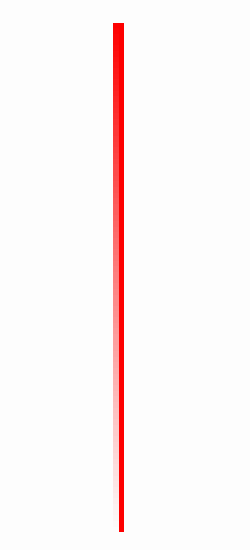
\includegraphics[height=8cm]{linie_aproximativ_verticala.png}
    \centering
    \caption{Linie aproximativ verticală}
    \label{fig-linie-verticala}
\end{figure}

\begin{figure}[ht]
    
\includegraphics[height=5cm]{linie_oblica.png}
    \centering
    \caption{Linie înclinată la 45 de grade}
    \label{fig-linie-oblica}
\end{figure}

\subsection{Cum tratez liniile orizontale?}

Un caz particular al acestei metode este reprezentat de liniile orizontale. Conceptual nu are sens ca o linie
orizontală să aibă acoperiri ai pixelilor. Acest lucru nu ar face posibilă calcularea sumei cumulative în mod corect.
De exemplu, dacă fiecare pixel de pe o linie orizontală ar avea acoperire \(100\%\), suma cumulativă ar deveni egală
cu numărul de pixeli. Această sumă este mult prea mare pentru a se putea ajunge înapoi la 0 pentru delimita figura.
Astfel, desenarea s-ar face în mod incorect.

Soluția este să ignor liniile orizontale. O figură bine definită va avea mereu segmente care nu sunt orizontale,
acestea dictând suma cumulativă. În cazul triunghiului desenat în figura \ref{fig-triunghi-simplu}, baza are acoperirile
dictate de linia oblică din stânga. Biblioteca acceptă doar figuri bine definite, adică figuri închise, similar cum SVG
acceptă doar figuri închise pentru algoritmii de umplere.

\chapter{Extinderea algoritmului la mai multe primitive}

Pentru a facilita desenarea figurilor mai complexe, am extins algoritmul de bază, adăugând suport pentru curbe Bézier
de ordin 2 și ordin 3. Ideea implementării este de a converti curbele la o înșiruire de linii suficient de „densă” pentru
a nu se putea observa faptul că de fapt am desenat niște linii, și nu am lucrat analitic cu curbele.

\section{Curbe Bézier de ordin 2}

Curbele Bézier de ordin 2 sunt reprezentate sub forma:

\[
    B(t) = (1 - t)^2 P_0 + 2 (1 - t) t P_1 + t^2 P_2, \ 0 \leq t \leq 1
\]

Unde \(P_0, P_1, P_2\) sunt punctele de control ale curbei.

Pentru a converti curbele Bézier de ordin 2 la linii am ales să implementez metoda prezentată de Raph Levien
\cite{FlatteningQuadraticBezierCurves}. Metoda propusă prezintă o formulă pentru calcularea numărului de segmente
necesare pentru a reprezenta curba, folosindu-se de proprietatea curbelor Bézier de ordin 2 care ne spune că acestea
pot fi interpretate ca o secțiune dintr-o parabolă \(y = x^2\), modulo rotație, scalație și translație.

Distanța maximă între curbă și coardă pentru o parabolă \(y = x^2\) este aproximativ \(\frac{1}{8} \kappa \Delta s^2\),
unde \(\kappa\) reprezintă curbura iar \(\Delta s\) reprezintă o distanță tinzând spre 0, astfel considerând o coardă cât mai mică.
Formulele pentru acestea, pentru o parabolă, sunt relativ simple:

\[
    \kappa = \frac{f''(x)}{\left(1 + f'(x)^2\right)^{\frac{3}{2}}} = \frac{2}{\left(1 + 4x^2\right)^{\frac{3}{2}}}
\]
\[
    \Delta s = \sqrt{1 + \left(\frac{dy}{dx}\right)^2} dx = \sqrt{1 + 4x^2} \Delta x
\]

Înlocuind acestea în formula de mai sus putem determina pe \(\Delta x\):

\[ \Delta x = 2 \sqrt{\Delta y} \sqrt[4]{1 + 4 x^2} \]

Care reprezintă „pasul” necesar pentru fiecare linie. Pentru a afla numărul de segmente vom calcula inversul aceste expresii,
luat pe intervalul pe care îl dorim:

\[
    f(x) = nr. segmente = \frac{1}{2 \sqrt{\Delta y}} \int\limits_{x_0}^{x_1} \frac{1}{\sqrt[4]{1 + 4x^2}} dx
\]

Pentru determinarea parametrului \(t\) pentru fiecare linie generată, va trebuie să calculăm inversul acestei funcții. Metoda
propusă oferă două aproximări pentru calcularea acestora:

\[
    f(x) \approx \frac{x}{0.33 + \sqrt[4]{0.67^4 + \frac{1}{4} x^2}}
\]
\[
    f^{-1}(x) \approx x \left( 0.61 + \sqrt{0.39^2 + \frac{1}{4} x^2} \right)
\]

În implementare se folosește o structură care să faciliteze lucrul cu curbele Bézier de ordin 2, așa cum este prezentată în
figura \ref{fig-struct-quadbezier}. Convertirea la linii, prezentată în \ref{fig-quadbezier-subdivide}, se efectuează folosind
ideea prezentată mai sus. După cum se poate vedea, algoritmul nu este recursiv, spre deosebire de metoda De Casteljau
care este folosită de obicei.

\begin{figure}[ht]
    \centering
    \begin{lstlisting}[language=Rust]
pub struct QuadraticBezier {
    x0: f64, y0: f64,
    x1: f64, y1: f64,
    x2: f64, y2: f64
}
    \end{lstlisting}
    \caption{Structura care descrie curbele Bézier de ordin 2}
    \label{fig-struct-quadbezier}
\end{figure}

\begin{figure}[ht]
    \centering
    \begin{lstlisting}[language=Rust]
pub fn subdivide(&self, err: f64) -> Vec<f64> {
    let params = self.map_to_basic();
    let (a0, a2) = (
        approximate_integral(params.x0),
        approximate_integral(params.x2)
    );
    let count = 0.5 * f64::abs(a2 - a0)
        * f64::sqrt(params.scale / err);
    let n = f64::ceil(count);
    let (u0, u2) = (
        approximate_inverse_integral(a0),
        approximate_inverse_integral(a2)
    );
    let mut result = vec![0_f64];

    for i in 1..(n as i32) {
        let u = approximate_inverse_integral(
            a0 + ((a2 - a0) * (i as f64)) / n
        );
        let t = (u - u0) / (u2 - u0);
        result.push(t);
    }

    result.push(1.0); return result;
}
    \end{lstlisting}
    \caption{Algoritmul de convertire a curbelor Bézier de ordin 2 la linii}
    \label{fig-quadbezier-subdivide}
\end{figure}

În figura \ref{fig-curba-bezier-de-ordin-2} se poate vedea un exemplu de curbă Bézier de ordin 2 desenată folosind metoda
prezentată mai sus, cu un parametru de toleranță de \(0.5\) - parametru care decide cât de „aproape” de curba ideală vrem
să fim; cu cât valoarea este mai mică cu atât curba va arăta mai „curbată”, dar se vor genera și mult mai multe linii și
performanța poate scădea. Poza este mărită intenționat pentru a observa calitatea implementării. Deși în figură se poate observa
faptul că doar am generat linii în loc să desenez o curbă, în practică acest lucru este aproape invizibil, mai ales când
se desenează text. Curbele vor fi oricum mici sau nu vor avea astfel de curburi extreme. Arăt acest fapt prin figura
\ref{fig-litera-arond}. Am desenat-o cu un parametru de toleranță chiar mai mare, adică \(1.0\), și se poate observa cum
este invizibil faptul că s-au generat linii pentru a desena curbele care constituie litera „@”.

\begin{figure}[ht]
    \includegraphics[height=5cm]{curba_bezier_de_ordin_2.png}
    \centering
    \caption{O curbă Bézier de ordin 2}
    \label{fig-curba-bezier-de-ordin-2}
\end{figure}

\begin{figure}[ht]
    \includegraphics[height=10cm]{litera_arond.png}
    \centering
    \caption{Litera „@” desenată folosind metoda menționată}
    \label{fig-litera-arond}
\end{figure}

\section{Curbe Bézier de ordin 3}

Pentru a converti curbele Bézier de ordin 3 la linii am folosit algoritmul lui De Casteljau, mai exact metoda
prezentată de Kaspar Fischer \cite{DeCasteljau_algorithm}. O curbă Bézier de ordin 3 este reprezentată ca:

\[
    B(t) = (1 - t)^3 P_0 + 3 (1 - t)^2 t P_1 + 3 (1 - t) t^2 P_2 + t^3 P_3, \ 0 \leq t \leq 1
\]

Unde \(P_0, P_1, P_2, P_3\) sunt punctele de control ale curbei Bézier de ordin 3.

Algoritmul lui De Casteljau ne dă o metodă prin care să împărțim curba la un anumit \(t\) în 2 curbe mai mici,
de același ordin. Metoda menționată vine cu o metodă de a decide când să ne oprim să împărțim curba în două,
adică când considerăm că linia curentă este suficient de mică astfel încât efectul vizual să fie cât mai bun.
În figura \ref{fig-cubic-split} prezint codul care se ocupă cu această evaluare, care se folosește la rândul
ei de un parametru de toleranță.

\begin{figure}[ht]
    \centering
    \begin{lstlisting}[language=Rust]
// is_sufficiently_flat
let mut u = 3.0 * p1 - 2.0 * p0 - p3;
let mut v = 3.0 * p2 - 2.0 * p3 - p0;

ux *= u.x; u.y *= uy;
vx *= v.x; v.y *= vy;

if u.x < v.x {
    u.x = v.x;
}
if u.y < v.y {
    u.y = v.y;
}

let is_flat = ux + uy <= tolerance;
    \end{lstlisting}
    \caption{Instrucțiunile care decid când o linie este suficient de mică pentru a ne opri în împărțirea De Casteljau}
    \label{fig-cubic-split}
\end{figure}

Generarea liniilor este implementată printr-un algoritm recursiv, descris în \ref{fig-subdivision-algorithm}.

\begin{figure}[ht]
    \centering
    \begin{lstlisting}[language=Rust]
fn subdivide(&self, lines: &mut Vec<Point>, tolerance: f64) {
    if self.is_sufficiently_flat(tolerance) {
        lines.push(Point {
            x: self.x3,
            y: self.y3,
        });

        return;
    }
    let (left, right) = self.split();
    left.subdivide_impl(lines, tolerance);
    right.subdivide_impl(lines, tolerance);
}
    \end{lstlisting}
    \caption{Algoritmul care convertește curbe Bézier de ordin 3 la linii}
    \label{fig-subdivision-algorithm}
\end{figure}

În figura \ref{fig-cubic-example} se poate vedea o demonstrație a metodei de desenare a curbelor Bézier de ordin 3.
Parametrul de toleranță folosit pentru generare a fost \texttt{0.25}. Din nou, faptul că am folosit linii pentru a „simula”
curba este practic vizual invizibil.

\begin{figure}[ht]
    \includegraphics[height=8cm]{curba_cubica.png}
    \centering
    \caption{Figură determinată de mai multe curbe Bézier de ordin 3}
    \label{fig-cubic-example}
\end{figure}

\newpage

\section{Desenare de text}

Având implementarea pentru primitivele mai sus menționate, pot desena text prin desenarea de caractere descrise prin
fonturi precum TrueType. Caracterele sunt descrise prin curbe Bézier, eu trebuind doar să traduc descrierea din formatul
TrueType în formatul pe care îl acceptă proiectul meu. Pentru acest lucru mă ajut de pachetul \texttt{ttf\_parser}
\cite{TrueTypeParser}.

Acest pachet îmi va citi un fișier TrueType și îmi va permite să implementez cinci funcții care vor fi folosite pentru
traducerea descrierii caracterelor din formatul TrueType în formatul bibliotecii mele, așa cum este demonstrat în figura
\ref{fig-ttf-parser-demo}. Am prezentat doar funcția \texttt{move\_to}, dar implementarea se adaptează ușor la celelalte funcții.
Există câte o funcție pentru fiecare primitivă din enumerarea \texttt{PathOps} prezentată de mine la început. În figurile
\ref{fig-text-verg} și \ref{fig-text-fmi} se pot vedea două exemple de text desenat folosind biblioteca mea. Figura
\ref{fig-text-verg} a fost generată folosind fontul Roboto \cite{Roboto}, iar figura \ref{fig-text-fmi} a fost generată
folosind fontul Wildwood \cite{Wildwood}.

\begin{figure}[ht]
    \centering
    \begin{lstlisting}[language=Rust]
fn move_to(x: f32, y: f32) {
    let new_point = Point {
        x: (x - min_x) as f64,
        y: height as f64 - (y - min_y) as f64,
    };
    prev_point = new_point;
    starting_point = new_point;
    path_ops.push(PathOps::MoveTo {
        x: new_point.x,
        y: new_point.y,
    });
}
    \end{lstlisting}
    \caption{Funcția \texttt{move\_to} folosită de \texttt{ttf\_parser}}
    \label{fig-ttf-parser-demo}
\end{figure}

\begin{figure}[ht]
    \includegraphics[width=5cm]{text_verg.png}
    \centering
    \caption{Numele bibliotecii mele desenat folosind chiar biblioteca}
    \label{fig-text-verg}
\end{figure}

\begin{figure}[ht]
    \includegraphics[height=5cm]{text_fmi.png}
    \centering
    \caption{Textul „FMI” desenat folosind biblioteca mea}
    \label{fig-text-fmi}
\end{figure}

\chapter{Efecte}

Pentru a permite descrierea figurilor mai complexe, am implementat în bibliotecă și suport pentru efectul de gradient.
Mai concret, am implementat suport pentru gradienți liniari, radiali și conici, care vor fi descriși în detaliu mai jos.
De asemenea, am introdus și suport pentru diverși operatori de amestecare, adică operatorii Porter-Duff \cite{Porter-Duff}.
Se pot introduce inclusiv funcții de amestecare care să fie definite de utilizator, pentru flexibilitate maximă. În plus,
am adăugat suport și pentru transformări afine asupra punctelor care constituie figurile.

\section{Gradienți}

\subsection{Liniari}
\subsection{Radiali}
\subsection{Conici}

\section{Amestecare}
\subsection{Porter-Duff}

\section{Transformări}

\section{Spații de culoare}

\chapter{Concluzii}

\printbibliography

\end{document}